\chapter{New Material}
\chapterauthor{Jeff Yoshimi}

This document contains notes for additions that will eventually be made to the book, in particular to supplement changes and new features in Simbrain 4. Chapter and section headings correspond to where in the book the new material will be placed. This material is very rough. Corrections. and comments welcome.

\section{New Material for Linear Algebra Chapter}

% TODO: Pictures for source-target representations
 
\subsection{The scalar and vector tracks}

% Compare https://youtu.be/Smav86u60FM?t=390 (from neurons to tokens, from weighted combinations of scalars to weighted combinations of vectors)

%To get to the next belt level, you have to deal with this kind of thing, and so train your brain to deal with it.

The book  can be thought of as involving two tracks: a `scalar' and a `vectorized' track. In the scalar track, we think of all operations from the standpoint of individual neurons and their values. We index weights using a source-target structure. In Simbrain, the focus is mostly on separately presented nodes. We use vectors and matrices to understand many ideas conceptually, but we do not make heavy use of matrix products or matrix algebra. This is much more accessible to beginning students, and is sufficient to teach an entire class. Indeed, this has been the way the book was structured and is the main way Simbrain 3.0 works. This supports the main thrust of the book and Simbrain, making neural networks easy enough to use without any math background at all (there is math to learn, but it is self contained). 
% Source target entails a different representation of matrices

However, this is not how things are done by most professionals working on neural networks in industry, and most academics as well (ch 1 taxonomy). For any serious work, we must move to the vectorized approach. Everything becomes more concise, and runs more efficiently on high performance performance computers. This requires a change in thinking, a way of seeing and thinking about these problems in terms of matrices, vectors, and tensors, often seeing datasets and batches in new ways, almost as tubes of information that get transformed. The focus here is on vectors, matrices, and higher rank tensors, and on applying linear algebra methods directly to these structures. The weights are now indexed using a target-source scheme. The basic objects are mostly matrices, and matrix products--especially multiplications of matrices by column vectors--are the basic operations. In Simbrain 4.0 we have been and are making efforts to make this mode of thinking more intuitive. As of now, there is very little in this format in the book, but we are in the process of adding chapters and sections that present that point of view. Ultimately the hope is to have enough material that a more advanced course could be done entirely from that point of view.

One downside of this is that the indexing changes depending on what you read, but we hope this downside can be an upside. The main book allows a non-math approach, but those going to the target-source point of view must also develop an ability to switch between representations, to see it both ways, which is more complex cognitively but in a way that suits the more advanced mind sets. Many problems are like that, allowing for multiple representations.

% Define shape of matrix
% Transposes.  Also address in line vectors and whether they need the transpose. There's this weird situation. In simbrain and in general, the default is columns.   But in a book, the default is row.  So to show column we do transose operator. But if bold face alone, it is colulmn

\subsection{Graphical conventions}

To think in terms of vectors, we need to bridge between conventional linear algebra notation, and conventional neural network representations, as in Simbrain.  We need a template for mentally moving back and forth between these ways of thinking.  

The first thing to do is get clear on the shape of the matrix. Remember, we are using an ``output-input'' representation.  It feels backwards but it's how it's done.  So, in figure \ref{linalgToSimbrain}, start on the right with Simbrain.  Count the number of outputs, then the number of inputs. Then we have an output-input matrix.  So $3$, $2$, and a $3 \times 2$ matrix.

\begin{figure}[h]
\centering
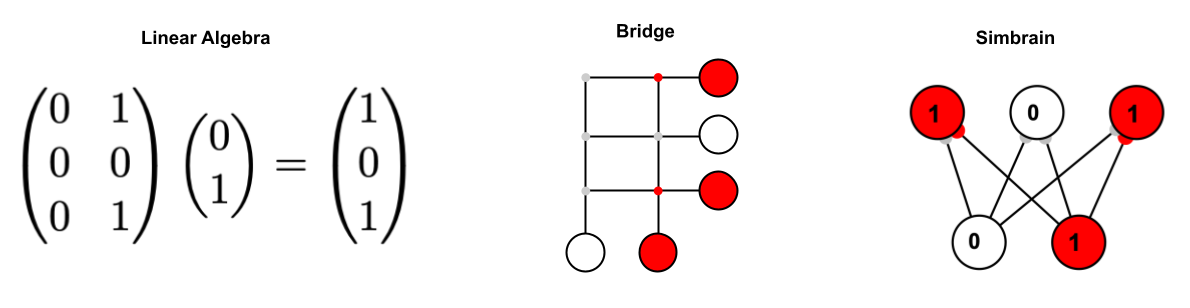
\includegraphics[width=0.75\textwidth]{images/LinalgToSimbrainReps.png}
\caption[Jeff Yoshimi.]{A set of images to help link standard visual representations in linear algebra (left) with standard visual representations of neural networks (right), via the intermediate representation in the middle. }
\label{linalgToSimbrain}
\end{figure}

Figure \ref{linalgToSimbrain} is an effort to bridge this gap. On the left is a standard matrix product, $\mathbf{W} \mathbf{x} = \mathbf{y}$.  This is how forward propagation of an input vector through a weight matrix is usually understood. The weight matrix is $\mathbf{W}$, the input is $\mathbf{x}$, and the output is $\mathbf{y}$. We think of the matrix as operating on the column vector to produce a new column vector.   

% need a transpose section
Here is how I suggest you think about this to connect it up to intuitions about neural networks.  Think of the column vector $\mathbf{x}$ as being rotated 90 degrees or transposed to become a row vector (imagine grabbing the vector by the $1$ and pulling it up and to the right). Now mentally take this row and move it to the bottom of the weight matrix, as in the middle panel of  \ref{linalgToSimbrain}. The weight matrix and the output vector stay in the same orientation.  The fan-out weight vectors from the input are shown as vertical lines, and the fan-in weight vectors to the output are shown as horizontal lines. Now we can easily ``follow'' the activations upwards as activity is propagated. 
% The bridge is pretty close to the new simbrain rep. Show that?
% Note there are other reps too, like the points in a space rep.

I like to think of the input vector as being dotted with each fan-in weight vector on the outputs to produce the entries of the output vector.

To go from the bridge to the standard Simbrain representation in the right panel we now leave the inputs in place, and imagine the outputs being rotated 90 degrees and moved to the top, and imagine the weights kind of following along. Hopefully you can just see it. 

In Simbrain 4.0, we have designed the representation of activation vectors and weight matrices to follow the ``bridge'' concept above as closely as possible.  See figure \ref{simbrain4_ff23}.

\begin{figure}[h]
\centering
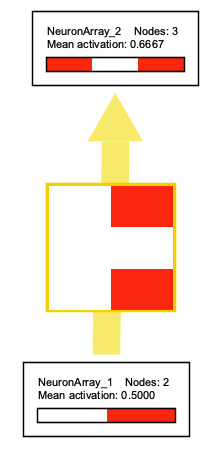
\includegraphics[width=0.15\textwidth]{images/simbrain4_ff_2_3.png}
\caption[Jeff Yoshimi.]{Graphical conventions for activation vectors and weight matrices in Simbrain 4. }
\label{simbrain4_ff23}
\end{figure}
%
%Also just a thought on how to think about the weight matrices. Their shape is target-source, or output-input. So if we have a 3-5-2-1 network in terms of node layers, we have three weight matrices. Their shapes are:
%
%5x3
%2x5
%1x2
%
%So you would pass a list of the form [5x3, 2x5, 1x2] to your function. Remember, weight matrices on the left are multiplied by input and activations vectors on the right.I find this pretty counter-intuitive and takes me a lot of practice to think in this “output-input” way.  I want to read left-to-right input-to-output but the standard conventions with matrix product reverse this...

\section{New Material for LMS / Backprop Chapter}

There are a lot of great technical discussions of this (citations). But the goal here in this book is intuition, trying to get a \emph{feel} for these things, so you can reason about them and think about how they might apply to cognitive science. 

(Most of this can be removed since it's already been added to the main chapter, but some stuff is still different so leaving it here for now).

Our goal in this chapter is the backprop model. That's the crown jewel. All other models can be thought of as instances of that one model. It is used to train feed forward networks using gradient descent. From Rosenblatt up to GPT 3, all models are variants on it. It's a big class. But here is some of the history.

\subsection{The Algorithm}

Now we can describe the LMS rule, and verify that it causes the weights to change a such a way that the sum of squared errors (SSE) gets lower over time.

% TODO: But no activation function yet
When applying the rule, a change in a weight $w_{i,j}$ is equal to the product of a learning rate $\epsilon$, the activation of the input node to that weight, $a_i$, and the difference between a desired and actual activation ($t_j - a_j$) for that node:
\begin{eqnarray*}
\Delta w_{i,j}  =  \epsilon a_i (t_j - a_j)
\end{eqnarray*}
Since $(t_j - a_j)$ is error  (with a small ``e''), the rule says that the change in a weight is equal to a learning rate times the activation of the input node for that weight, times the error. This should make some intuitive sense. As we saw above in the goldilocks discussion, for positive inputs weights should be changed in the direction of error. The input scales things so they work for positive or negative inputs and so that changes are bigger for bigger inputs, and the learning rate allows us to control how quickly learning happens. 

LMS also changes the bias $b_j$ of an output node $j$ as follows: 
\begin{eqnarray*}
\Delta b_j  =  \epsilon (t_j - a_j)
\end{eqnarray*}
That is, the change in a bias for a node $j$ is just the learning rate times the error on output node $j$.\footnote{Note that this is really the same as the weight change rule, if we think of the bias in terms another input neuron, clamped at 1, and attached to this output neuron by a modifiable weight (which is in effect the bias).}

Applying the rule involves two stages at each iteration. First, a ``forward pass'', where we compute the output of the network for a given input pattern. This is the normal activation update we've been talking about in past chapters, for a feed-forward network. We set the inputs, and apply the update rules to get the output activations. In our simple case here the main thing we are getting is just the activations $a_j$.  With multi-layer  networks we will propagate through many layers to get all the hidden activations and finally the output activation. 

% Backward refs
Second, a ``parameter update'' pass. At this point we have an  input-output pair, an ``output dataset'' with one row.  This allows us to compare the actual output with the target value, and compute error. We can then use this error $ (t_j - a_j)$ to apply the rule and get weight and bias update values, which we then apply to all the parameters, all the weights and biases.\footnote{With one weight layer networks using LMS this is simple, but later with many layered networks there is a bit more involved, and in fact there is a process of multiplying the errors backwards through the weights, which is a kind of ``backward pass'' and where the name ``backpropagation'' comes from.}

We are in the scalar case of one output node, and just considering one input-output pair. But the full algorithm involves changing many output nodes, and doing it for many output pairs.  We have also not considered what happens when the output activation function is something besides unbounded linear. We'll add these cases step by step in the chapter, but it's helpful to start off simple.

% Talk about how divergence looks in this kind of case. And add some practice examples that show it happening. E.g. Given a1 = -3, w12=4, t = 0, epsilon = 1, what is w12'?

\subsection{The Algorithm: Intuition}

The plan here will be to give an intuitive feel for the algorithm in a simple case, and then to derive it, and then to add in the details (bias and activation functions) as optional sections, and then to do it for the vector case.

We start with scalar values, the case of a single target. We have a bunch of data, saying what the network did (outputs) and what we wanted it to do (targets). So we have error, but where the rows have one column for output and one for target. So our error is just one value. The error is target value minus the actual output, $e = t-a$. These errors are the main thing to think about at first. 

Think of this as a  {\bf Goldilocks principle}: just as someone might keep heating and cooling porridge until it is just right--way too hot, cool it a bunch, oh now a bit too cold, heat it a bit, ahh now just right. stop changing things... we increase and decrease parameters until overall error is just right.\footnote{A useful picture showing how this method leads to a decision boundary that correctly classifies all training examples is here: \url{https://commons.wikimedia.org/wiki/File:Perceptron_example.svg}.} The math ends up making this work.

%Intuitively, the algorithm works like this (for positive valued inputs). If the output is too high, the error is negative. For example, if I wanted 4 but got 5, error is $4-5 = -1$. I have to make the weights and bias a little bit lower to make the output lower. On the other hand, if the output is too low, the error is positive. For example, if I wanted 5 but got 4, error is $5-4 = 1$. I have to make the weights and bias a little larger. (Notice that multiplying the weights by the error would send us in the right direction, and that larger errors will lead to larger weight changes). If the output is just right, don't change anything. By incrementally changing the weights and biases in this way, the network slowly learns to produce the correct response to all inputs.
 
Recall the rule:
\begin{eqnarray*}
\Delta w_{i,j}  =  \epsilon a_i (t_j - a_j)
\end{eqnarray*}
Since $(t_j - a_j)$ is error  (with a small ``e''), the rule says that the change in a weight is equal to a learning rate times the activation of the input node for that weight, times the error. This should make some intuitive sense in Goldilocks terms. Let's consider each factor of this rule: the error and the source activation, separately.

% Wait, cohere this with the fact that we go opposite the gradient. It's in the derivation sectio but cohere it here.
First, the error tells us what direction to change the parameters in, which makes sense:
\begin{enumerate}
\item Positive error. Example target is 2 and output is 1. Error is $2-1 = 1$. The output is too low, so we need to make the weight larger. The porridge was too cold, so we need to make it hotter. 
\item Negative error. Example target is 0 and output is 1. Error is $0-1 = -1$. The output is too large, so we need to make the weight smaller. The porridge was too hot, so we need to make it cooler. 
\end{enumerate}

But we also end up multiplying by the source value? Why? Well, think about it, again in the two cases.
\begin{enumerate}
\item Large source activation. This is making a big change in the output. So we want any change to be proportional. The output was too high, and this source activation is large, so we want to make the change in the weight also large, to compensate for the big activation
\item Small source activation. The output was too high, but this source activation was not big, so we just change things a bit. It's contributing less to the problem.
\end{enumerate}
Also, negative source activations will make the weight change change sign as well, so that we make changes in the right direction. % TODO: Examples

This is like a variant on the Hebb rule. Hebb said, just change the weight based on the product of source and target. Fire together wire together. That has use for detecting patterns of correlation between input and output. Make the output reflect those correlations. But now we say something different. We change weight based on the product of source activation and the error. We in a sense correlate with the error, which reduces the error, until the error is close to 0.

One last way to think of this is in terms of statistical concepts. We can think of LMS as repeatedly testing the network and correcting for false positives (the output is too high; a ``type 1'' error) and false negatives (the output is too low; a ``type 2'' error) until the error rate is as low as possible. This analysis makes mmost sense for classification tasks with binary variables.
 \subsection{Computing error surfaces}

A brief interlude to discuss these error surfaces, like the one in \ref{error_lms} and how the algorithm ends up going down the gradient. It may help to think about how that was created? Since we were only looking at a single target value and error relative to a single weight, it can actually be computed by hand. In the example, squared error is

\begin{eqnarray*}
(t - a_2)^2 =  (t - (a_1 w_{1,2} + b_2))^2 = (t - a_1 w_{1,2})^2  
\end{eqnarray*}
We can ignore bias because bias is 0.

Now think about all possible values for the weights. Remember, we want to find a value for the weight that will minimize our error. So we can just substitute the actual output activation $a_j$ above with the expression for it, which is source activation times weight, or  $a_1 w_{1,2}$.

\begin{eqnarray*}
(t_j - a_1 w_{1,2})^2
\end{eqnarray*}

So now we can substitute in the values from our example:

\begin{eqnarray*}
(2 - 1 * w_{1,2})^2 = \\
(2 - w_{1,2}) (2 - w_{1,2} ) =  \\
4-4w_{1,2}+w_{1,2}^2
\end{eqnarray*}
This tells us, for any given value of $w$, what the squared error will be. That is what is plotted in the figure. Gradient descent using the LMS rule will find the weight value that minimizes the error.

However, computing this all by hand can be  a pain, especially as we consider more parameters and a larger training set, so you can also make a little computer program to do it.  Here is the idea. Make a function

%\subsection{Code for an error function}
%
%(These subsections put the code in a separate place. Rather than psuedocode, we'll use python code, which is like executable pseudocode)
%
%Rather than working out an equations like this every time imagine we have a function that take an output dataset, a weight, and bias, and returns the sum of the squared error. Here is some python code that does that, for a case where the output dataset just has one input per row, where 0 is the index for the first column (inputs) and 1 is the index for the second column (targets):
%
%\begin{center}
%\begin{minipage}{0.5\textwidth}
%\begin{verbatim}
%def sse(dataset, weight, bias):
%    error = 0
%    for row in dataset:
%        aj = row[0] * weight + bias
%        tj = row[1]
%        row_error = tj - aj
%        error += row_error * row_error
%    return error
%\end{verbatim}
%\end{minipage}
%\end{center}
%
%You can use this code with a fixed weight value and an array of bias values to produce an error surface for biases, or a fixed bias value and an array of weight values to produce an error surface for weights (that is what we did above for a bias of 0), or pass in an array of both weights and biases and then plot a 2d error surface for weights and biases both.

%	Exercises
%	- Mod the script so that it shows how error changes with training set. Try to find a set where min error is not 0
%	- Mod it again to show error on a 2d surface
%	- Mod it again to show error with respect to bias (add in the bias discussion and note how simple it is)

\subsection{Bias intuition}

Here is the bias update rule again. Change the bias $b_j$ of an output node $j$ as follows: 
\begin{eqnarray*}
\Delta b_j  =  \epsilon (t_j - a_j)
\end{eqnarray*}
That is, the change in a bias for a node $j$ is just the learning rate times the error on output node $j$.\footnote{Note that this is really the same as the weight change rule, if we think of the bias as another input neuron, clamped at 1, and attached to this output neuron by a modifiable weight (which is in effect the bias).}

This one really makes sense in terms of Goldilocks. If the output is too high, make the bias smaller, if it is too low, make the bias higher. It does not respond to inputs, so you can't usually train a network on bias alone, but it does get the adjustments right. An exercise you can do is trying to update the bias only, the weights only, and then both (as the algorithm does), just by coding this all up and then commenting out the bias update line and the weight update line in your code. See how it does in each case.

\subsection{Derivation of the LMS rule}

All this can be shown using calculus. It's kind of amazing to turn the crank on the calculus, and see how it all works out giving us the rule above, with all the intuitive meaning. Run through the calculus, and we get our rule, which we saw above makes sense!

Conceptually, we are using the derivative of the error space. Since it's multi-dimensional, we call the derivative a gradient in this case. The gradient is a vector that points in the direction of change. 

We want to change the weight so that error is reduced. Let's leave the bias out for now. Then we are taking this derivative:

\begin{eqnarray*}
\frac{dE}{dw_{1,2}} (t - a_2)^2
\end{eqnarray*}

Recall that $a_2 =  a_1 w_{1,2} + b_2$. Substituting, we get
\begin{eqnarray*}
\frac{dE}{dw_{1,2}} (t - ( a_1 w_{1,2} + b_2))^2 
\end{eqnarray*}

Using the chain rule (derivative of the outside part applied to the inside part, times the derivative of the inside part), and substituting again, we get

\begin{eqnarray*}
\frac{dE}{dw_{1,2}} = 2 (t - a_1 w_{1,2} - b_2) (-a_1) =   2 (t - a_2) (-a_1)  = -2 a_1 (t - a_2)
\end{eqnarray*}

And since $t - a_2$ is error $e$ we get

\begin{eqnarray*}
\frac{dE}{dw_{1,2}} = -2 e a_1
\end{eqnarray*}

This says that the change in error with respect to the weight is given by error times source activation times a constant. The 2 can be ignored, since we can think of it as being absorbed into the learning rate. Also, this gradient points in the direction of error increasing. But we want to go in the opposite direction, so that error is reduced. So we multiply this gradient by $-1$, changing its sign. And so our learning rule is 

\begin{eqnarray*}
\Delta w_{1,2}  =  \epsilon a_1 e  = \epsilon a_1 (t - a_2)
\end{eqnarray*} 

Of course this generalizes, and so our general learning rule for weights is:
\begin{eqnarray*}
\Delta w_{i,j}  =  \epsilon a_i (t_j - a_j)
\end{eqnarray*} 

As an exercise, try deriving the rule for bias. The setup is

\begin{eqnarray*}
\frac{dE}{db_{2}} (t - ( a_1 w_{1,2} + b_2))^2 
\end{eqnarray*}

Now let's add in the activation function $f$ and derive the weight-update rule.  This involves a few applications of the chain rule:

\begin{eqnarray*}
\frac{dE}{dw_{1,2}} (t - f(a_1w_{1,2} + b_2))^2   = 2 (t - f(a_1w_{1,2} + b_2)) f'(a_1w_{1,2} + b_2) a_1 
\end{eqnarray*}
Note that the derivative of the activation function $f'$ is like a free parameter here. Whatever your activation function $f$ is, to use gradient descent we just plug in $f'$ and we can do gradient descent. BUT some derivatives have problems, like being undefined or 0, which effectively turns off update.

Subbing in $a_2 = f(a_1w_{1,2} + b_2))$, and recalling $n_2 = w_{1,2} + b_2$ 

\begin{eqnarray*}
\frac{dE}{dw_{1,2}} (t - a_2)^2   = 2 (t - a_2) f'(n_2) a_1 
\end{eqnarray*}

So the learning rule for weights is:
\begin{eqnarray*}
\Delta w_{i,j}  =  \epsilon a_i (t_j - a_j) f'(n_j)
\end{eqnarray*} 

This is the same as before, but multiplied by with the derivative of the activation function applied to to the net input (the weighted input to the node). We discuss this more below.

Intuitively, the idea is to scale the rate of weight change by how much the activation function is changing things. So when the activation function is changing things a lot, we want the weight to change a lot too. When it changes things very little, the derivative is small and so we change the weight less.  It doesn't matter as much.  Also note that if the derivative is 0, then learning stops. That can be a problem with piecewise linear and relu activation functions, and is why the threshold activation function can't be used at all.  Again see below.

\section{Vector approach to LMS}

% TODO: Write some new material just for the new representation

In the scalar approach to LMS we multiply a single output error (target - output) by source activation. Now we have a vector of errors times a vector of source activations. But how to deal with indexing?  The algorithm is ultimately a variant on Hebb, so we already have a template for thinking about it.

The error part itself is easy, first we do target - output using elementwise subtraction: $\mathbf{t} - \mathbf{a}_{\text{out}}$.  To multiply these errors times source activations, we do the same thing as in Hebb: we multiply an $m \times  1$ column output errors times a $1 \times  n$ row of source activations to get an $m \times n$ matrix of weight deltas.  Then we scale that by learning rate, and add to the weight matrix.  (There remains the issue of the bias, and any activation functions on the output, but we're starting simple.) So, the vectorized rule is
\begin{eqnarray*}
\Delta \mathbf{w}  =  \epsilon (\mathbf{t} - \mathbf{a}_{\text{out}}) \mathbf{a}_{\text{in}}^T
\end{eqnarray*}
Remember, by default all vectors in bold face are column vectors.  So this is a column vector (the error $\mathbf{t} - \mathbf{a}_{\text{out}}$) times a row vector (the input activations) which produces a matrix in the same shape as the weight matrix.

Consider the network shown in figure \ref{lms_vector_pre}.

\begin{figure}[h]
\centering
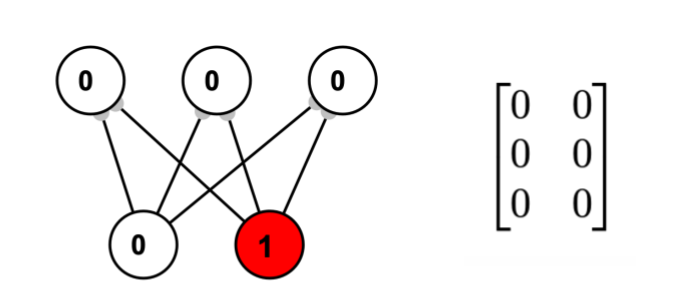
\includegraphics[width=0.55\textwidth]{images/vectorLMSBeforeTrain.png}
\caption[Jeff Yoshimi.]{A network with empty weights. We want it to learn to associate $(0,1)$ input to $(1,0,1)$}
\label{lms_vector_pre}
\end{figure}

Remember, the weight matrix is a 3x2 matrix  (``target-source''), which we are treating as all zero in this example. Each row is a fan-in of an output node, and the columns are fan-outs of input nodes. Our template for thinking about this is to imagine inputs coming up from the bottom, and dotting with the fan-in weight vectors to produce outputs (really net-inputs, to which bias is added and an activation function applied)

Our values are
\begin{equation*}
\epsilon = 1 \; \; \\
\mathbf{a}_{\text{in}} = \begin{bmatrix} 0 \\ 1 \end{bmatrix} \\
\mathbf{t} = \begin{bmatrix} 1 \\ 0 \\ 1 \end{bmatrix}
\mathbf{a}_{\text{out}} = \begin{bmatrix} 0 \\ 0 \\ 0 \end{bmatrix}
\end{equation*}

Then the equation is learning rate times error times input transposed:

\begin{align*}
\Delta \mathbf{w}  = 1
\begin{bmatrix} 1 \\ 0 \\ 1 \end{bmatrix} 
\begin{bmatrix} 0 & 1 \end{bmatrix} 
= \begin{bmatrix} 1 \cdot 0 & 1 \cdot 1 \\ 0 \cdot 0 & 0 \cdot 1 \\ 1 \cdot 0 & 1 \cdot 1 \end{bmatrix} 
= \begin{bmatrix} 0 & 1 \\ 0 & 0 \\  0 & 1  \end{bmatrix}
\end{align*}

So we get

\begin{align*}
\mathbf{w} + \Delta \mathbf{w}  =
\begin{bmatrix} 0 & 0 \\ 0 & 0 \\  0  & 0  \end{bmatrix} +
\begin{bmatrix} 0 & 1 \\ 0 & 0 \\  0  & 1  \end{bmatrix} =
\begin{bmatrix} 0 & 1 \\ 0 & 0 \\  0  & 1  \end{bmatrix}
\end{align*}

And again, keeping in mind that rows are fan-in of output and columns are fan-out of input we get figure \ref{lms_vector_2}.

\begin{figure}[h]
\centering
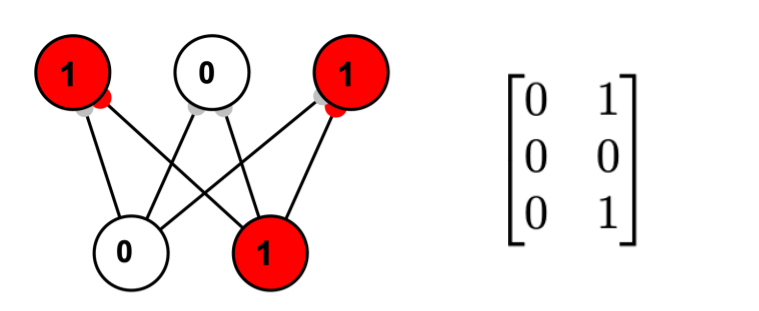
\includegraphics[width=0.55\textwidth]{images/vectorLMSAfterTrain.png}
\caption[Jeff Yoshimi.]{The network after training}
\label{lms_vector_2}
\end{figure}

We can now check that it works. Remember, think of the column vector on the right as ``entering'' from below, and dotting with each fan-in weight vector (each row of the matrix) to produce the output.  SSE has gone to 0 in a single time step.

\begin{align*}
\begin{bmatrix} 0 & 1 \\ 0 & 0 \\  0  & 1  \end{bmatrix}
\begin{bmatrix} 0 \\ 1 \end{bmatrix}
= \begin{bmatrix} 1 \\ 0 \\ 1  \end{bmatrix}
\end{align*}

% Add exercizes here, use Mak and David examples.
So now I suggest you try some examples of your own.  Come up with your own training set, apply the rule and see if you can run this a few times.  

\subsection{Bias}

To add bias updates in, we just vectorize the bias update rule, which has the same form as the scalar rule, since it's just elementwise.

\begin{eqnarray*}
\Delta \mathbf{b}  =  \epsilon (\mathbf{t} - \mathbf{a}_{out})
\end{eqnarray*}

So at each iteration, we change the bias vector just in the direction of the error vector. Remember goldilocks.  When things are too hot, cool them down. Etc.

\subsection{Activation functions}

(This material can also be added to the scalar case)


The full LMS rule also involves a derivative on the activation function.  These derivatives can be understood pretty intuitively if we look at those again. See figure \ref{derivativesActFunctions}.  The derivative for the threshold function is 0 everywhere except at the threshold where it is undefined (this was a problem for Rosenblatt). The derivative for the piecewise linear is 0 above and below the upper and lower bounds and the slope (usually 1) of the function in between those bounds. For the sigmoid it's close to what it is for piecewise linear, approaching 1 as net input is large or small and the slope at the inflection point in the middle, but we do need a formula for it.

\begin{figure}[h]
\centering
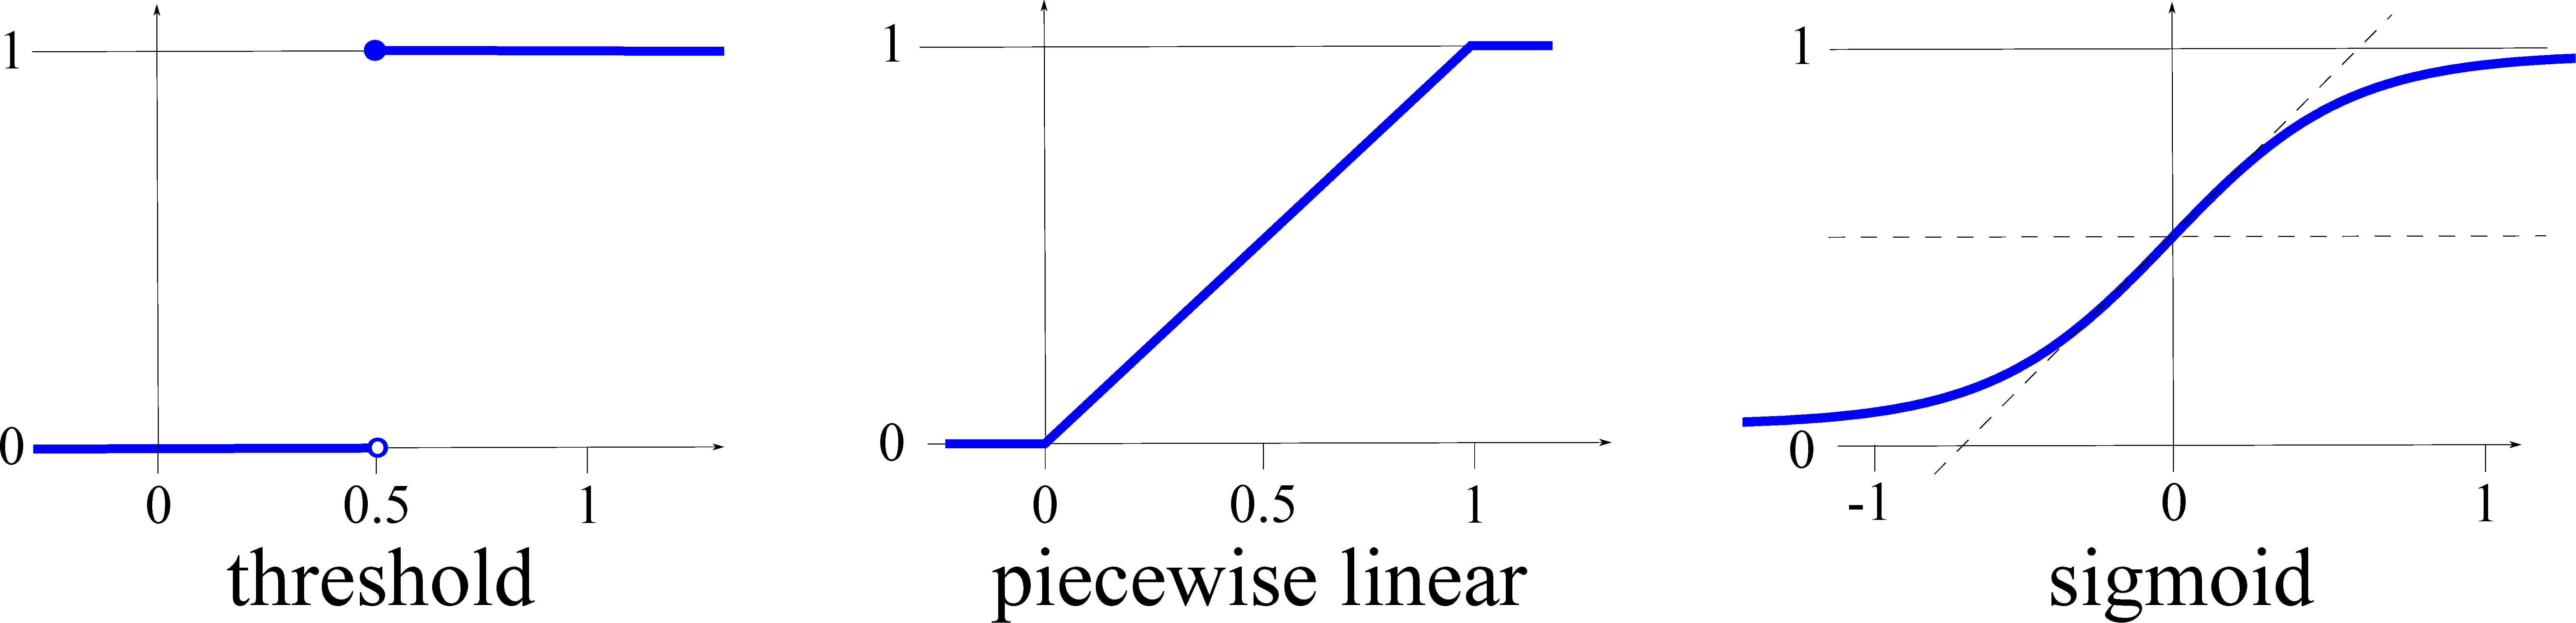
\includegraphics[width=0.75\textwidth]{images/graph_binary.pdf}
\caption[Jeff Yoshimi.]{The activation functions. The derivative is either 0 or the slope or close to the slope in most cases. }
\label{derivativesActFunctions}
\end{figure}

So how to work this into the LMS error update?

First, recall from chapter \extref{ch_act_functions} that the weighted input to a node $j$ is denoted $n_j$. This is the same as the activation of a linear unit. Its weights times input activations plus a bias.  An activation function $f$ then transformed this weighted inputs, so that $a_j = f(n_j)$.  When we incorporate activation functions we have to keep $a_j$ and $n_j$ separate so just get that clear before moving on.

Ok, and recall from the derivation that error update with an activation function involves the same as before multiplied by with the derivative of the activation function applied to to the net inpu.  Intuitively it's like we scale the error that we use to scale the weights and biases with a factor corresponding to how much the activation function changes things.\footnote{This is a problem with RELU, known as the ``dying Relu" problem.}  It's also why Rosenbatt's perception was limited; binary are 0 derivative everywhere so their weights never change using this rule, and so he had to come up with a kind of ad hoc solution.

So  the full rule for weights is

\begin{eqnarray*}
\Delta w_{i,j}  =  \epsilon a_i (t_j - a_j) f' (n_j)
\end{eqnarray*}

And the full rule for biases is 

\begin{eqnarray*}
\Delta b_{j}  =  \epsilon b_j (t_j - a_j) f' (n_j)
\end{eqnarray*}

Do both of these at each time step to update the network.


\subsection{The Full Vectorized LMS rule}

Putting it all together, thevectorized rule is

\begin{eqnarray*}
\Delta \mathbf{w}  =  \epsilon (\mathbf{t} - \mathbf{a}_{\text{out}}) f'( \mathbf{n}_{\text{out}}) \mathbf{a}_{\text{in}}^T
\end{eqnarray*}

We take a column of errors (targets - outputs), and scale each component by the derivative of the activation function applied to the weighted inputs. Remember, weighted inputs is just one more quantity that each node has. When it's updated, it must compute that, and then use that to compute the activation value. So the node has both values, and so we can easily get components of this column vector: we have the target, the output activation, and the net input at any time, and that is enough to get us the column vector. We then matrix multiply that by a row of source activations and the result is a matrix of weight deltas with the right shape.

\begin{eqnarray*}
\Delta \mathbf{b}  =  \epsilon (\mathbf{t} - \mathbf{a}_{\text{out}}) f'( \mathbf{n}_{\text{out}})
\end{eqnarray*}

All of these vector operations should be familiar. For the application of $f$, it's just a matter of apply it to each component of the vector.  For example, if $f(x) = x+1$ then $f(1,2) = (2,3)$. $f'$ is just a function so it can be applied in this way to a vector.

\section{New Material for Hebbian Update}

We've seen how the Hebb rule works for scalar values. Nice and easy: if they fire together, wire together; source times target activations.  The situation is the same when we vectorize the rule, but now we have activation vectors $\mathbf{a}_{\text{in}}$ and $\mathbf{a}_{\text{out}}$, and we have to find a vector operations that ``lines up'' the right components of the two vectors so that we strengthen the right ones.  Here is a preview: multiply the output activation column vector times the input row vector (the input transposed, since we assume columns to start), and out pops what we're looking for. 

So, as usual in the vector world, things end up feeling kind of backwards, we multiply output times input rather than the other way around, and there is this mysterious transpose thrown in.  But if we go back to the ``bridge'' panel of the figure above, it ends up making sense. Figure \ref{vectorizedHebb} shows the idea. I like to start in the center panel, and then (to link to the linear algebra) think of the mentally moving the output vector to the left and moving the input vector to the top. Then we have a kind of outer product representation, and all the products kind of line up in the right way. 


\begin{figure}[h]
\centering
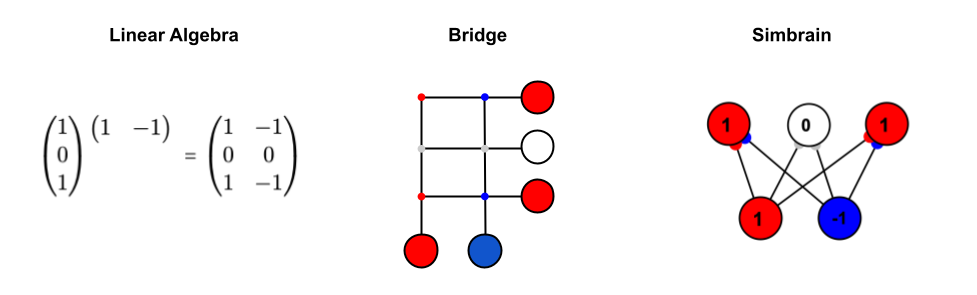
\includegraphics[width=0.9\textwidth]{images/vectorizedHebb.png}
\caption[Jeff Yoshimi.]{Using our visual conventions to conceptualized the vectorized Hebb rule,}
\label{vectorizedHebb}
\end{figure}

 As a slogan: output column times input row gives you a weight matrix.

As a sanity check in the example, check the shapes. We ahve a $3 \times 1$ output vector times a $1 \times 2$ row vectors, which gives us a weight matrix (or weight matrix delta) in the correct shape: $3 \times 2$. This is sometimes called an outer product.
So the vectorized Hebb rule is: 

% Be consistent about symbol for learning rate

Ok, so here is the vectorized Hebb rule:

\begin{eqnarray*}
\Delta \mathbf{w}  = \epsilon \mathbf{a}_{\text{out}} \mathbf{a}_{\text{in}} ^T
\end{eqnarray*}
Remember, by default all vectors in bold face are column vectors.  So this is a column vector (the output activation  $\mathbf{a}_{\text{out}}$) times a row vector (the input activations) which produces a matrix in the same shape as the weight matrix. Again, it feels backwards: we go from target to source (rather than source to target), just to get things in the right format.

The Hebb rule can also be vectorized. Suppose we have an input vector $\mathbf{x} = (1, -1)$, and an output vector $\mathbf{y} = (1,0,1)$. Remember, on an output-input representation, the weight matrix connecting them is $3 \times 2$. So our weight updates, assuming a learning rate of 1, correspond to all the connections between the entries in these two vectors. 

Here is an example
%\[
%\Delta \mathbf{w}  = 
%\begin{pmatrix} 1 \\ 0 \\ 1 \end{pmatrix}
%\begin{pmatrix} 1 & -1 \end{pmatrix}
%=
%\begin{pmatrix}
%    1 & -1 \\
%    0 & 0 \\
%    1 & -1
%\end{pmatrix}
%\]


Our values are
\begin{equation*}
\epsilon = 1 \; \; \; \; \\
\mathbf{a}_{\text{in}} = \begin{bmatrix} 1 \\ -1 \end{bmatrix} \\ 
\; \; \mathbf{a}_{\text{out}} = \begin{bmatrix} 1 \\ 0 \\ 1 \end{bmatrix}
\end{equation*}

Then the equation is (Once they are lined up like this it's kind of easy to ``see'' what is happening, especially in the bridge picture; all the cross points multiply)

\begin{align*}
\Delta \mathbf{w}  = 1
\begin{bmatrix} 1 \\ 0 \\ 1 \end{bmatrix} 
\begin{bmatrix} -1 & 1 \end{bmatrix} 
= \begin{bmatrix} 1 \cdot -1 & 1 \cdot 1 \\ 0 \cdot -1 & 0 \cdot 1 \\ 1 \cdot -1 & 1 \cdot 1 \end{bmatrix} 
= \begin{bmatrix} -1 & 1 \\ 0 & 0 \\  -1 & 1  \end{bmatrix}
\end{align*}

So we get

\begin{align*}
\mathbf{w} + \Delta \mathbf{w}  =
\begin{bmatrix} 0 & 0 \\ 0 & 0 \\  0  & 0  \end{bmatrix} +
\begin{bmatrix} -1 & 1 \\ 0 & 0 \\  -1 & 1  \end{bmatrix} =
\begin{bmatrix} -1 & 1 \\ 0 & 0 \\  -1 & 1  \end{bmatrix}
\end{align*}

Iterate again (assuming we are clamping the nodes; if we weren't the output activations would also be changing) and get


\begin{align*}
\mathbf{w} + \Delta \mathbf{w}  =
\begin{bmatrix} -1 & 1 \\ 0 & 0 \\  -1 & 1  \end{bmatrix} +
\begin{bmatrix} -1 & 1 \\ 0 & 0 \\  -1 & 1  \end{bmatrix} =
\begin{bmatrix} -2 & 2 \\ 0 & 0 \\  -2 & 2  \end{bmatrix}
\end{align*}

 Keep iterating and the entries at the top and bottom right will explode to positive infinity, and the top and bottom right will explode to negative infinity. This can be seen graphically in the Simbrain neuron array representation.
 
Try some other numbers and verify that as you repeatedly iterate, error will get smaller.

% TODO: Redraw a new pic just for vectorized hebb with all the right colors and values


\section{Backprop}

So this is the same thing, we take row error and use it the same way at the output row, but have to do a bit more work to get the hidden layers.

In terms of applications to cognitive science, there is this old work from Zipser that can be used to justify it!

\section{Batches}

This can all be done in pure linear algebra. But it can also be done in a looping way, that might be easier to learn. Then again good to be good with the weight multiplications. Not sure which is best. Maybe both?
